\hfuzz=100pt
\vfuzz=100pt
\subsection{Analyse}

Dette kapitel beskriver analyse, med tilhørende beslutninger og resultater.

\subsubsection{AnalyseKlassediagram} Ud fra de detaljerede brugsmønstre dannede gruppen et analyse klassediagram

\begin{figure}[H]
    %\centering
    \makebox[\textwidth][c]{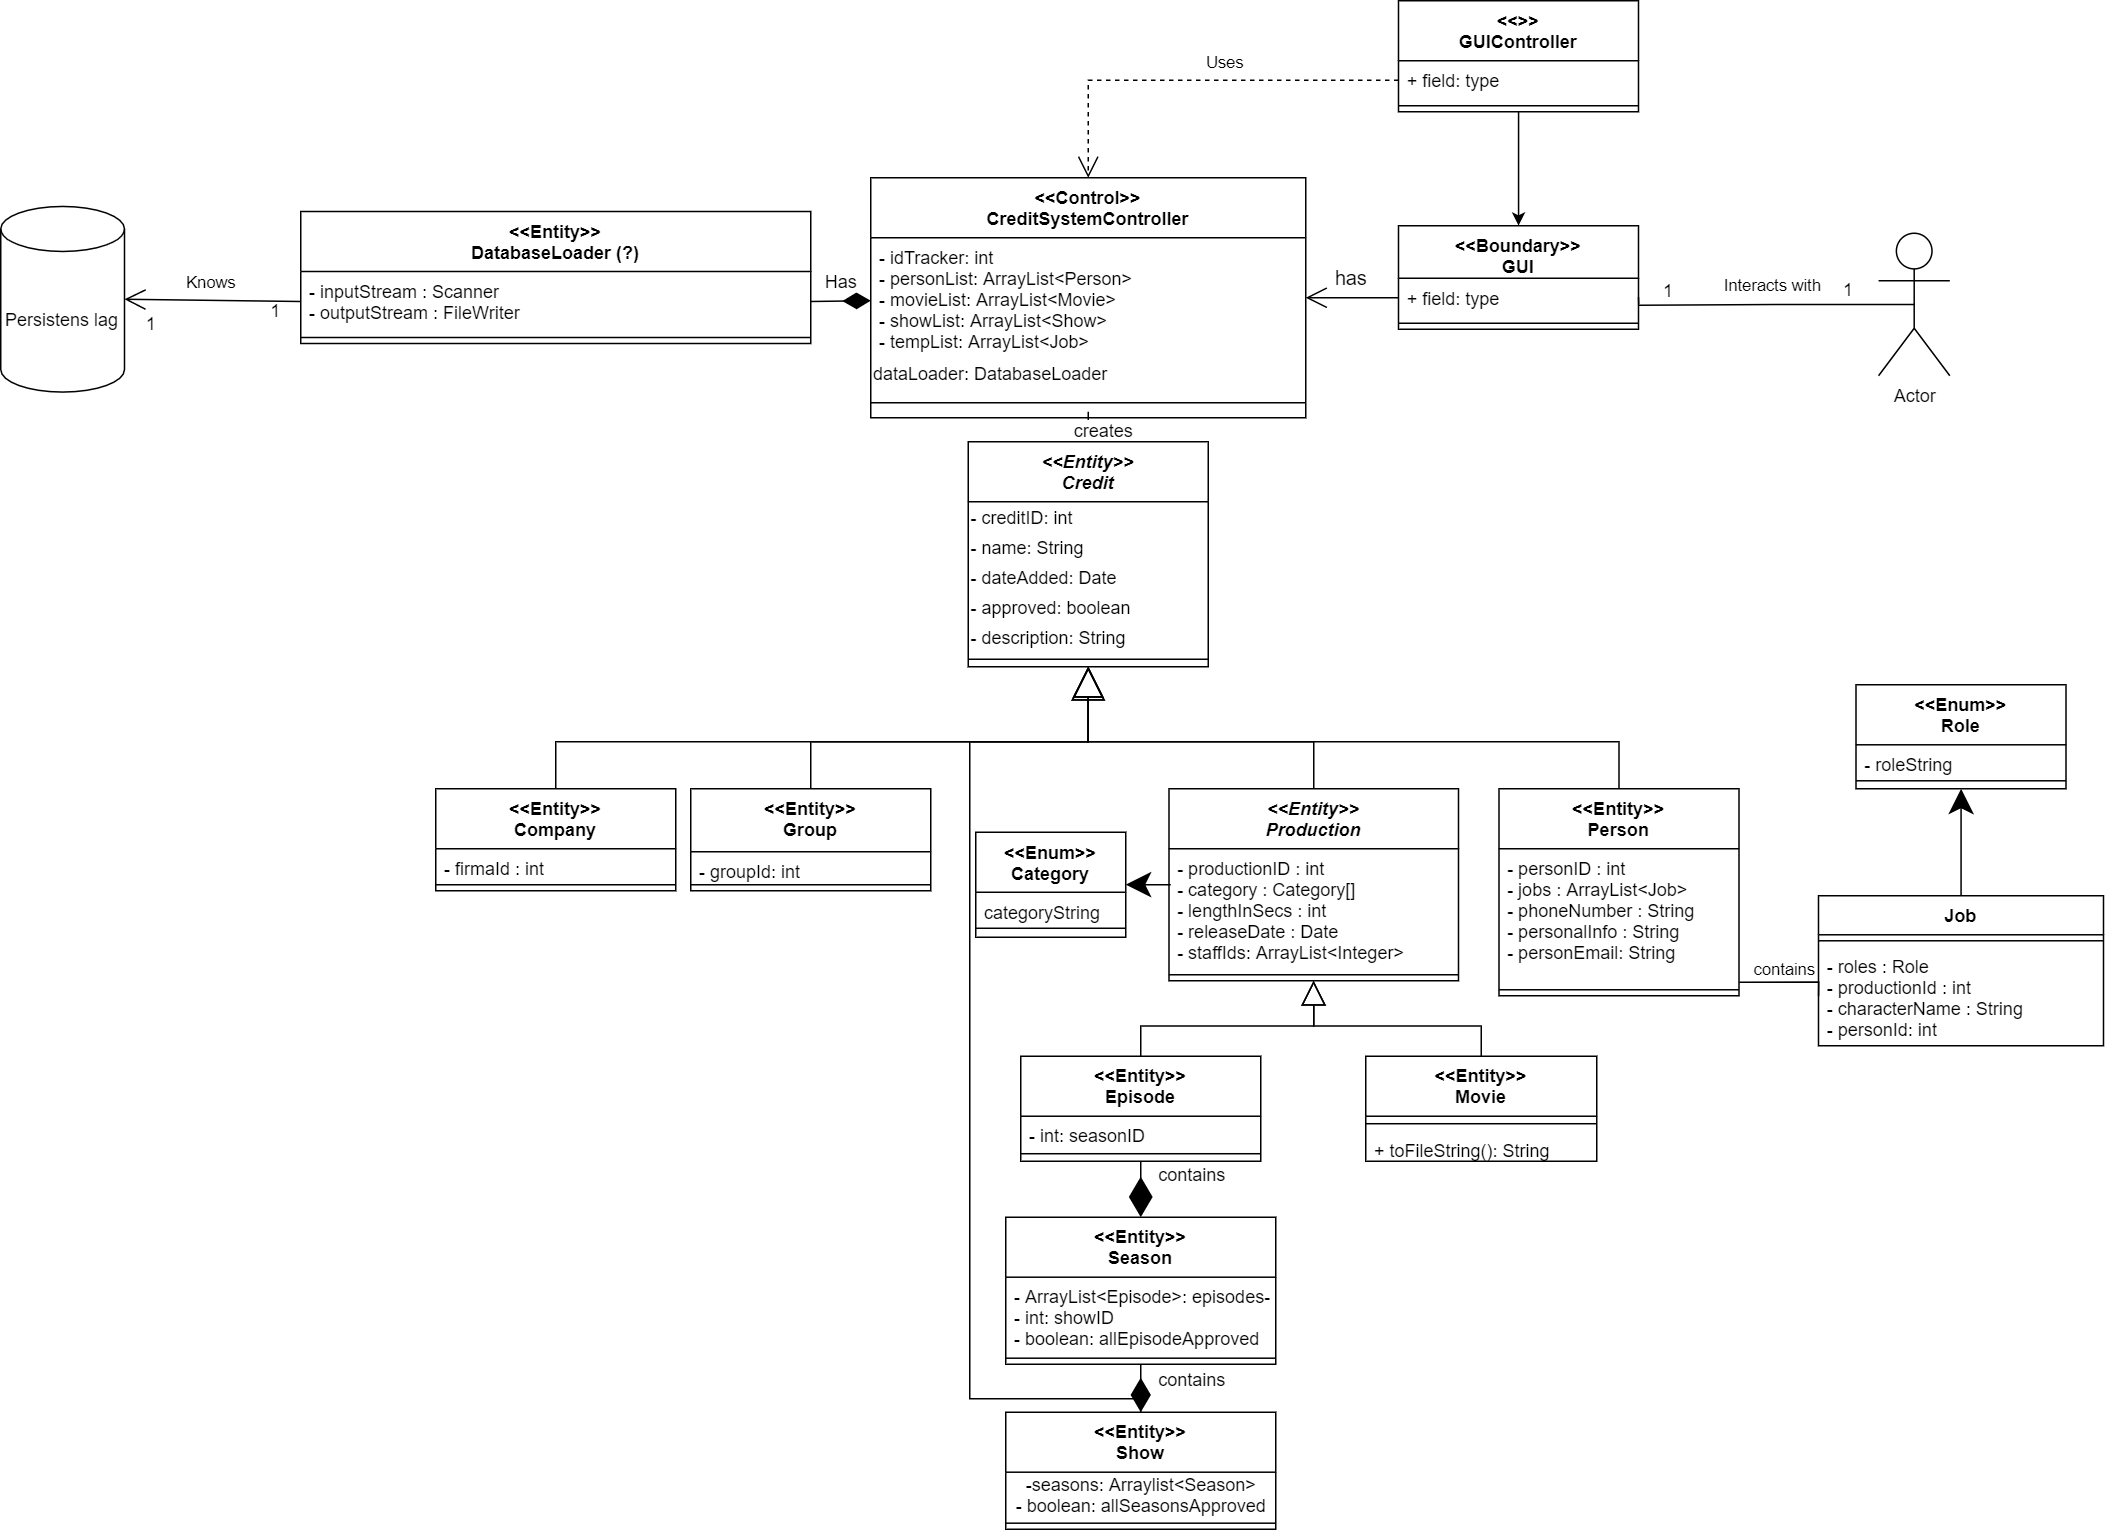
\includegraphics[width=1.2\textwidth]{images/AnalyseKlasseDiagram.png}}
    \caption{Analyse klasse diagrammet dannet fra de detaljerede brugsmønstre}
    \label{fig:AnalyseKlasseDiagram}
\end{figure}

Diagrammet viser den grundlæggende struktur. Centralt ligger en controller. Denne controller håndterer input fra GUI'en der har sine egen tilknyttede controllers, der håndterer interaktioner med knapper, tekstfelter osv. Den centrale controller skal blandt andet stå for at instantiere krediteringer. Dette bringer os til objekt-strukturen. Objekt strukturen er dannet ud fra både brugsmønstrene, og hvilke data TV 2 har opgivet skal inkluderes i systemet. Grundlæggende er alle indlæg i systemet en kreditering, og derfor vil alle (undtagen Job) nedarve fra Credit. Alle krediteringer vil have et navn, hvilken dato krediteringen er tilføjet, en beskrivelse og et overordnet creditID. Derudover markerer brugsmønsterdiagrammet også at en kreditering skal kunne godkendes og derfor at der tilføjet en boolean variabel navngivet approved. Fra Credit nedarver Group og Company, som ikke bærer noget ekstra information og får derfor kun et groupID og companyID. Disse to klasser er dog gennem projektet blevet nedprioriteret og er ikke blevet implementeret, så derfor vil der fremover ikke refereres til disse to. Person nedarver også fra Credit, og bærer noget personlig information som variabler. Systemet skulle også kunne holde film og serier. Ved dialog med Morten Lehm fra TV 2 Play, fandt gruppen frem til at, det at registrere hvad en person har bidraget til skal ske på episoden og ikke serien, da personalet kan variere fra episode til episode. Derved blev klassen Production tilføjet, da både Movie og Episode er en type af produktion, og derfor nedarver disse to fra den. En produktion har en kategori, som tilføjes via en enumerator kaldet Category, som indeholder alle kategorier som TV 2 har videregivet til gruppen i forbindelse med projektet. En episode kan dog ikke eksistere alene, men hører i stedet til en sæson. Ligesom episoden, kan en sæson heller ikke eksistere uden en serie, og derfor er der tilføjet komposition mellem disse klasser. Til sidst tilføjes job. Job er den klasse der markerer hvad en person har bidraget til, ved at samle personID og productionID i en klasse. Dette job er også markeret med en rolle, som tilføjes ved en Enum kaldet Role der indholder alle de roller som TV 2 har videregivet der skal krediteret. Fordelen ved at have denne Job klasse er at en person kan have flere job på samme produktion, hvis de f.eks. både var skuespiller og instruktør.
Analyse klassediagrammet ligger den grundlæggende struktur men er ikke nok til at starte implementeringen af programmet, da det ikke fortæller hvordan klasserne snakke sammen. Dette finde ved brugsmønsterrealisering

\subsubsection{Brugsmønsterrealisering} Formålet med brugsmønsterrealisering er at opfange opførslen af klasser, hvor klassediagrammet fortæller om forholdet mellem klasser. Efter brugsmønsterrealisering har man opnået et bedre overblik over hvilke metoder der kaldes hvor

\paragraph{B01: Registrering af kreditering} For at vise brugsmønsterrealisegingen af B01, tages der udgangspunkt i at tilføje en person. Operationerne vil stort set være det samme for andre typer af krediteringer, så derfor vises blot én af typerne for at visualisere det at registrere en kreditering.

\begin{figure}[H]
    \centering
    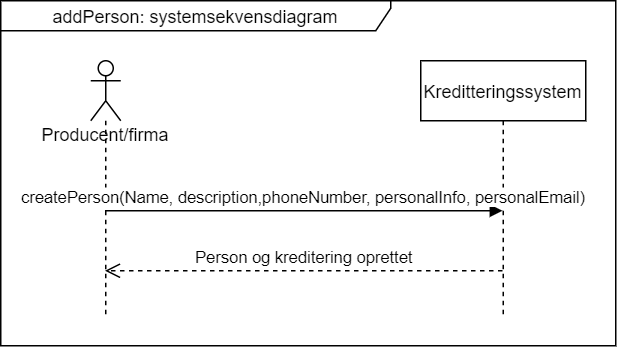
\includegraphics[scale = 0.5]{images/B01SSD.png}
    \caption{B01 Systemsekvensdiagram}
    \label{fig:B01_Systemsekvensdiagram}
\end{figure}

Figur \ref{fig:B01_Systemsekvensdiagram} viser et happy day scenarie for operationen addPerson. Når aktøren har interageret med systemet, skal der være tilføjet en ny person til filen eller Databasen. Der sendes navn ,beskrivelse, telefonnummer, personligtInfo og email. Dato indtastes ikke af brugeren, da systemet selv danner denne så der registreses den nøjagtige dato. Samtidig sættes approved variablen også automatisk til false, så den er klar til at blive tjekket igennem af en TV 2 moderator. Derudover er der også en idTracker der sørger for at der ikke opstår duplikerede ID. Denne vil dog blive udfaste ved brug af en relationel database, da den vil kunne struktureres med unikke ID som primaryKeys.  Ud fra dette diagram dannes en operationskontrakt.



\begin{table}[H]
\centering
\label{tab:2}
    \begin{tabular}{|p{35mm}|p{70mm}|} \hline
        \textbf{Kontrakt} &  \\ \hline
        \textbf{Operation} & addPerson(...) \\ \hline
        \textbf{Refererer til} & Brugsmønster: B01 Registrering af kreditering \\ \hline
        \textbf{Ansvar} & Ansvaret for denne operation at oprette en kreditering af type person med de indtastede oplysninger givet af aktøren fra GUI siden af. Operationen kræver at:
        \begin{itemize}
            \item Akøtren der vil tilføje en person har tilladelse til at tilføje krediteringer
            \item Der er indtastede informationer i de påkrævede felter. 
        \end{itemize}
        Når aktøren er færdig med at indtaste informationerne og vælger at registrere krediteringen skrives dette til persistenslaget
        \\ \hline
        \textbf{Prækonditioner} & Aktøren er logget ind som en bruger der har rettigheder til at registrere krediteringer\\ \hline
        \textbf{Postkonditioner} &
        En ny kreditering af type person er tilføjet og ligger i persistenslaget. Denne kreditering er ikke godkendt.\\ \hline
    \end{tabular}
        \caption{Operationskontrakt for operationen addPerson}
        \label{tab:OperationsKontraktB01}
\end{table}

Kontrakten har belyst nogle punkter der ikke er inkluderet i analyse klassediagrammet. En aktør skal f.eks. kun kunne registrere krediteringer hvis det er en bruger der har rettigheder til dette. Derved skal der foregår en form for tjek et sted i programmet. Det kunne være en variabel der ligger et sted i programmet så GUI'en kan tjekke om brugeren har lov, eller overhovedet får vist muligheden for at registrere krediteringer. Kontrakten belyser også at krediteringen skal godkendes af en der ikke er aktøren der tilføjer krediteringen. Det giver anledning til at der er en bruger der har flere rettigheder.
 
\begin{figure}
    \centering
    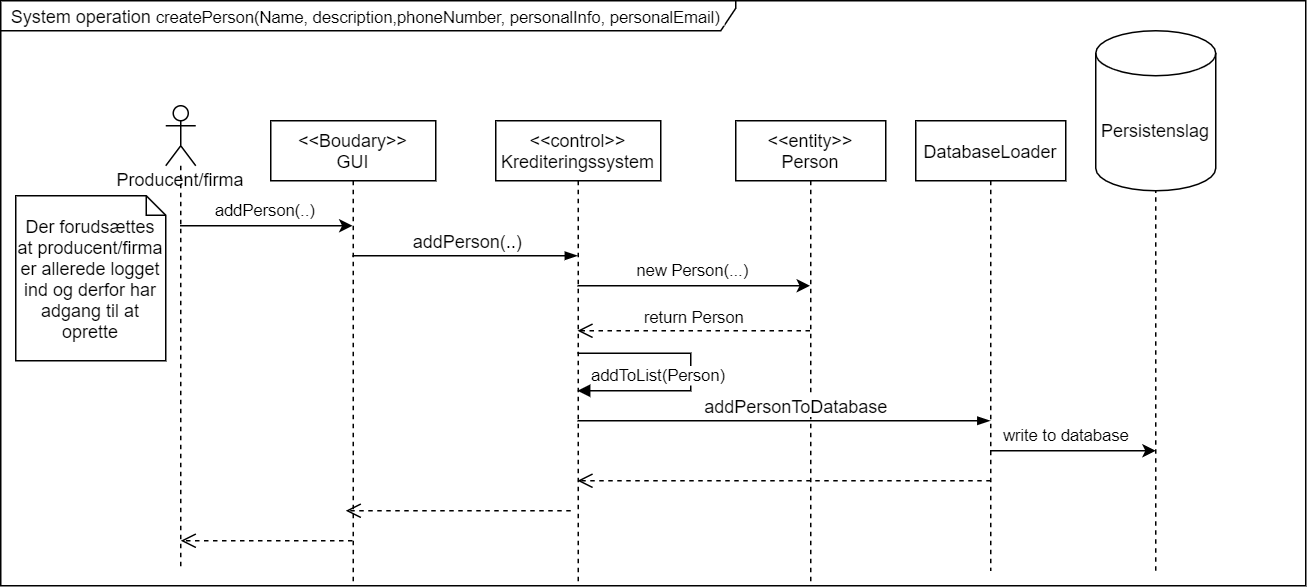
\includegraphics[scale = 0.37]{images/B01OSD.png}
    \caption{Sekvensdiagram for operation på B01}
    \label{fig:OperationsSekvensDiagramB01}
\end{figure}

Figur \ref{fig:OperationsSekvensDiagramB01} viser operationerne for at tilføje en person. Der er anvendt tre punktumer (...) i stedet for parameterene for at øge læsbarheden. Parameterene står oppe øverst i titlen på diagrammet. Som kontrakten på tabel \ref{tab:OperationsKontraktB01} angav, så forudsætter sekvensdiagrammet at aktøren er logget ind og har rettigheder. Hvis de har det, indtaster de informationerne i GUI, som videresendes til krediteringssystemControlleren der gennem Person klassen laver en ny instans, og returnerer denne til controlleren der sender personen videre til DatabaseLoaderen som skriver personen ind i filen/databasen.
Denne brugsmønsterrealisering resulterede i flere brugbare inputs. Der skal laves adgangskontrol og nuværende bruger skal opbeværes i systemet. Det blev taget en beslutning om at lave om på navngivningen af klassen der indtil videre er refereret til som CreditSystemController/Krediteringssystem. Denne bliver omdøbt til ApplicationManager da det er denne der styre meget af logikken i applikationen. Denne kommer også til at opbevare nuværende brugertype så der kan tjekkes om brugeren har de rette rettigheder. Til at tjekket disse rettigheder blev det besluttet at aktøren slet ikke skal få vist muligheden for at tilføje krediteringer hvis de ikke at logget ind som en der har rettigheder. Dette giver anledning til en login controller der knytter sig til GUI og sætter og får brugertypen på ApplicationManager. De opdaterede elementer på klassediagram vil så se ud som vis på figur \ref{fig:AnalyseKlasseDiagramV2}


\begin{figure}[H]
    \centering
    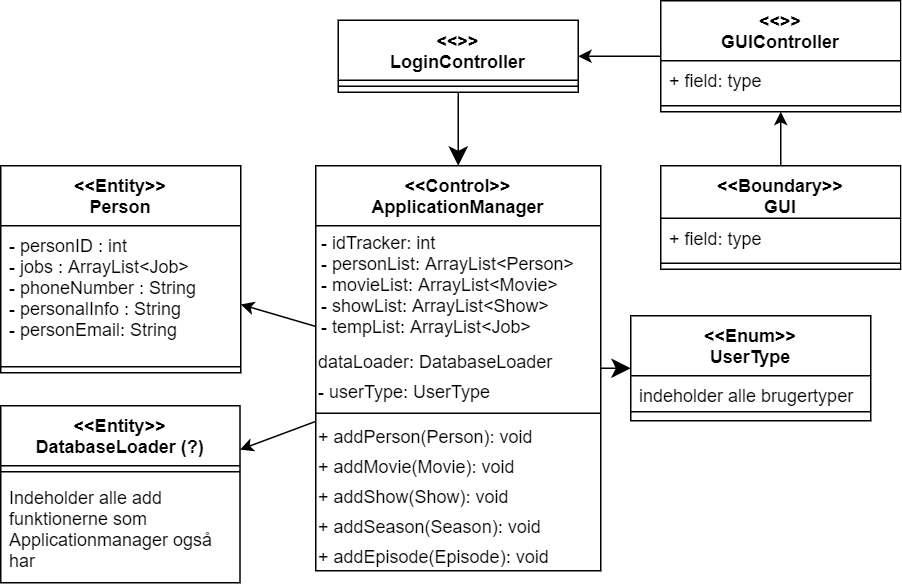
\includegraphics[scale = 0.4]{images/AnalyseKlasseDiagramV2.png}
    \caption{Revideret analyse klassediagram}
    \label{fig:AnalyseKlasseDiagramV2}
\end{figure}

\paragraph{B03: Foretage en søgning} Først dannes der et systemsekvensdiagram. Dette giver et overblik over hvad målet er. Systemsekvensdiagrammet for B03 ses på firgur \ref{fig:SystemsekvensdiagramSearch} 

\begin{figure}[H]
    \centering
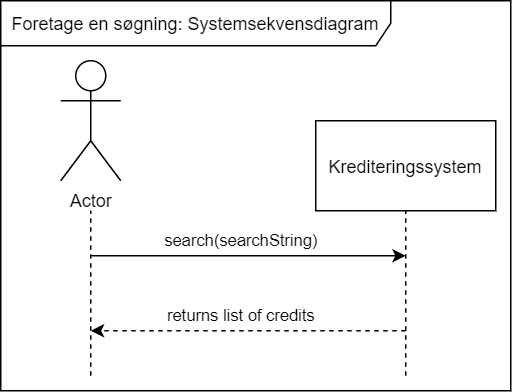
\includegraphics[scale = 0.5]{images/B03SSD.png}
    \caption{Systemsekvensdiagram for search}
    \label{fig:SystemsekvensdiagramSearch}
\end{figure}

Firgur \ref{fig:SystemsekvensdiagramSearch} viser at en aktør, her en bruger, bruger funktionen search på krediteringssystem som derefter returnerer en liste af krediteringer. Dette er happy day scenariet hvor aktøren får vist en liste af krediteringer, hvor den kreditering de søger er inkluderet.
Ud fra dette diagram blev der opsat en operationskontrakt over hvilket ansvar search operationen har. Denne operationskontrakt ses på tabel \ref{tab:OperationsKontraktB03}

\begin{table}[H]
\centering
\label{tab:2}
    \begin{tabular}{|p{35mm}|p{70mm}|} \hline
        \textbf{Kontrakt} &  \\ \hline
        \textbf{Operation} & search(searchString) \\ \hline
        \textbf{Refererer til} & Brugsmønster: Foretag en søgning \\ \hline
        \textbf{Ansvar} & Ansvaret for denne operation er at at modtage en forespørgsel fra en bruger og vise de krediteringer der svarer til forespørgslen, for brugeren hvis:
        \begin{itemize}
            \item Der eksisterer krediteringer der matcher brugerens forespørgsel
            \item Den ønskede kreditering er godkendt af TV 2 moderatorer 
        \end{itemize}
        Den liste som brugeren får vist, vil indeholde en mængde af krediteringer der passer til deres forespørgsel, og kunden kan her vælge en af disse krediteringer, og få yderligere information om den\\ \hline
        \textbf{Prækonditioner} & Databasen indeholder data\\ \hline
        \textbf{Postkonditioner} &
        Brugeren får vist en liste af krediteringer som matcher forespørgslen.\\ \hline
    \end{tabular}
        \caption{Operationskontrakt for operationen search}
        \label{tab:OperationsKontraktB03}
\end{table}

Tabel \ref{tab:OperationsKontraktB03} fortæller at ansvaret for search operationen er at finde de krediteringer der matcher brugerens forespørgsel, og returnere dem så de kan ses. Dette kræver at der er data det matcher i databasen som samtidig er godkendt af en TV 2 moderator. Der skal altså tilføjes funktonalistet til at tjekke om en kreditering er godkendt eller ej inden den vises. Instantieringen af objekter for at vise dem på GUI delen giver også anledning til nogle design valg. Man kunne instantiere dem med det samme man hente det fra databasen/filen, eller måske opbygge en service til instantieringen/konstruktionen af objekter. Kontrakten belyser i hvert fald flere muligheder i dette tilfælde
Herefter udarbejdede gruppen et sekvensdiagram for operationer inde i systemet som kan ses på figur \ref{fig:OperationsSekvensdiagramSearch} 
\begin{figure}[H]
    %\centering
\centerline{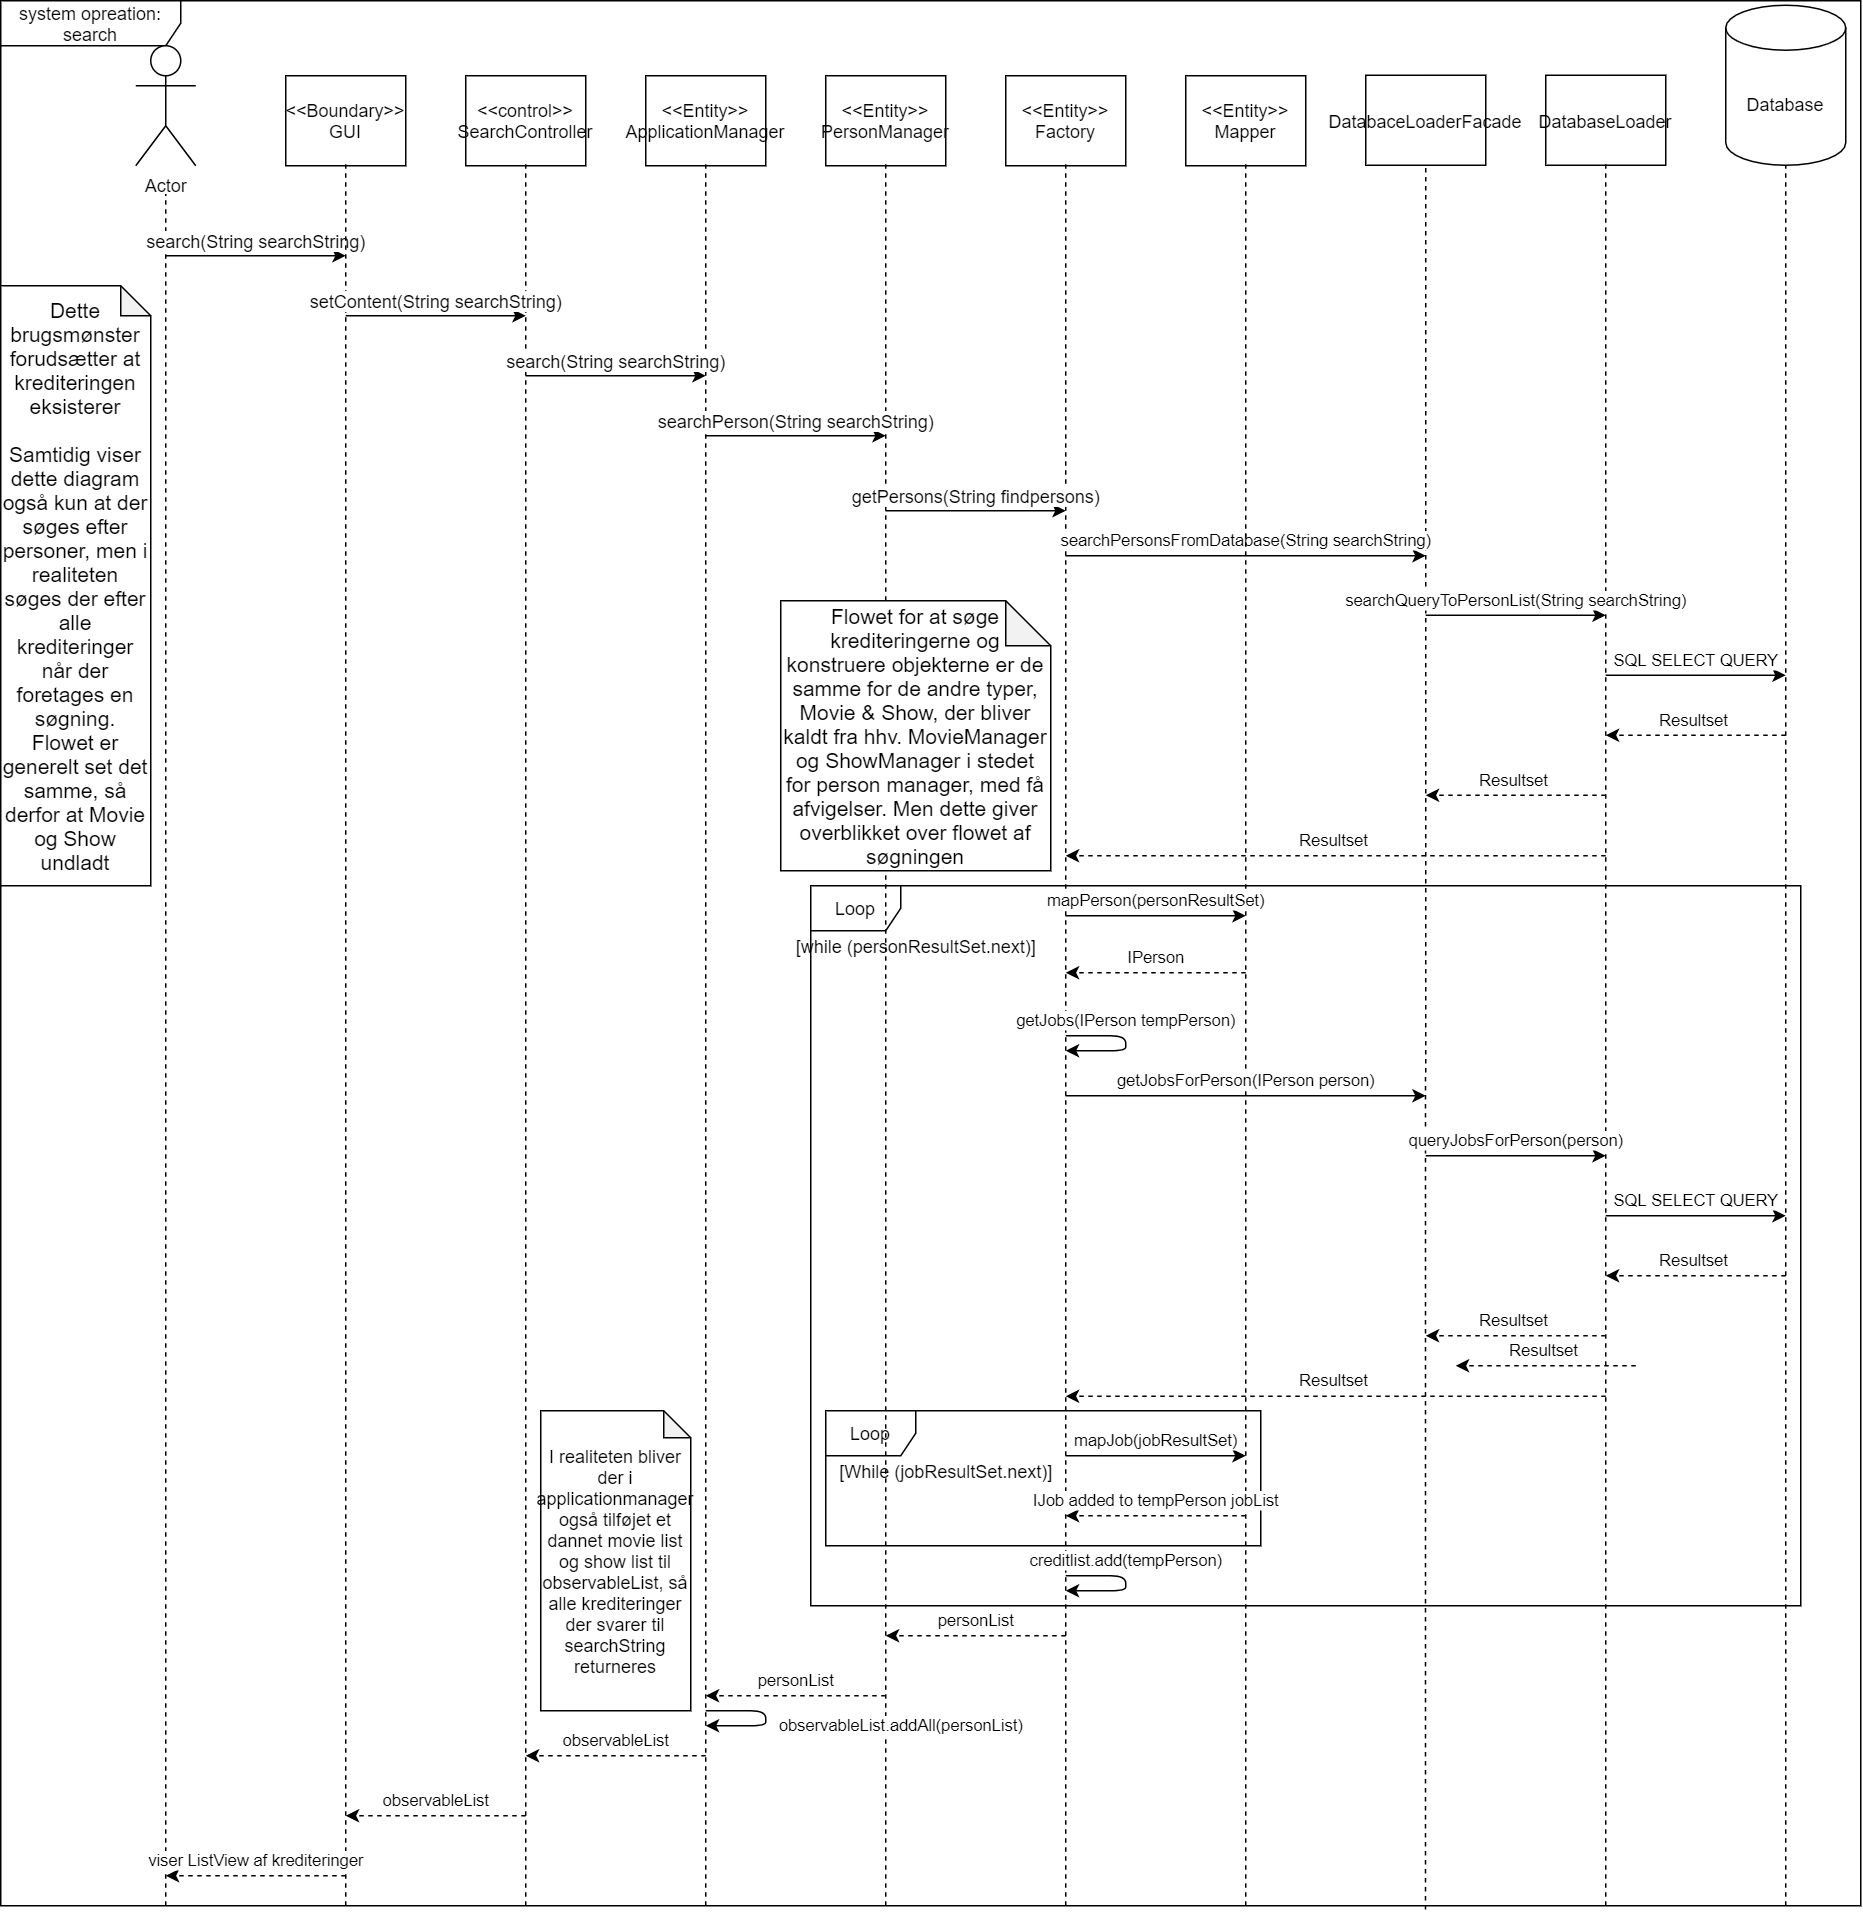
\includegraphics[scale = 0.37]{images/B03OSD.png}}
    \caption{Sekvensdiagram for operationer på search}
    \label{fig:OperationsSekvensdiagramSearch}
\end{figure}

Figur \ref{fig:OperationsSekvensdiagramSearch} viser operations sekvensdiagrammet for søgefunktionen search der bliver kaldt på GUI delen. GUI delen sender searchString som aktøren har indtastet videre til ApplicationManager der flere gange kalder DatabaseLoader. En gang for hver type af kreditering der er implementeret. DatabaseLoader queryer så filen/Databasen som sender resultatet tilbage til DatabaseLoader. Har opstår er par interessante designmuligheder. Man kunne instantiere objekter allerede nu, eller sende resultatet tilbage til ApplicationManager og instantiere dem her. Yderligere kunne man også lave en tjeneste der udelukkende står for at instantiere objekterne. Det giver mange muligheder som udforskes i designafsnittet. Fælles for alle metoderne er, at krediteringen skal tilføjese til en liste, og når alle krediteringer er kørt igennem, returneres listen, og i enden vises listen for aktøren.

Denne process gentages for resten af brugsmønstrene, for at danne et komplet analyse klassediagram, hvor der kan blive taget velbegrundede design beslutninger for at sikre en god software arkitektur. Efter brugsmønsterrealiseringsprocessen havde gruppen dannet følgende analyse klassediagram der ses på figur \ref{fig:AnalyseKlasseDiagramV3}.

\begin{figure}
    %\centering
\makebox[\textwidth][c]{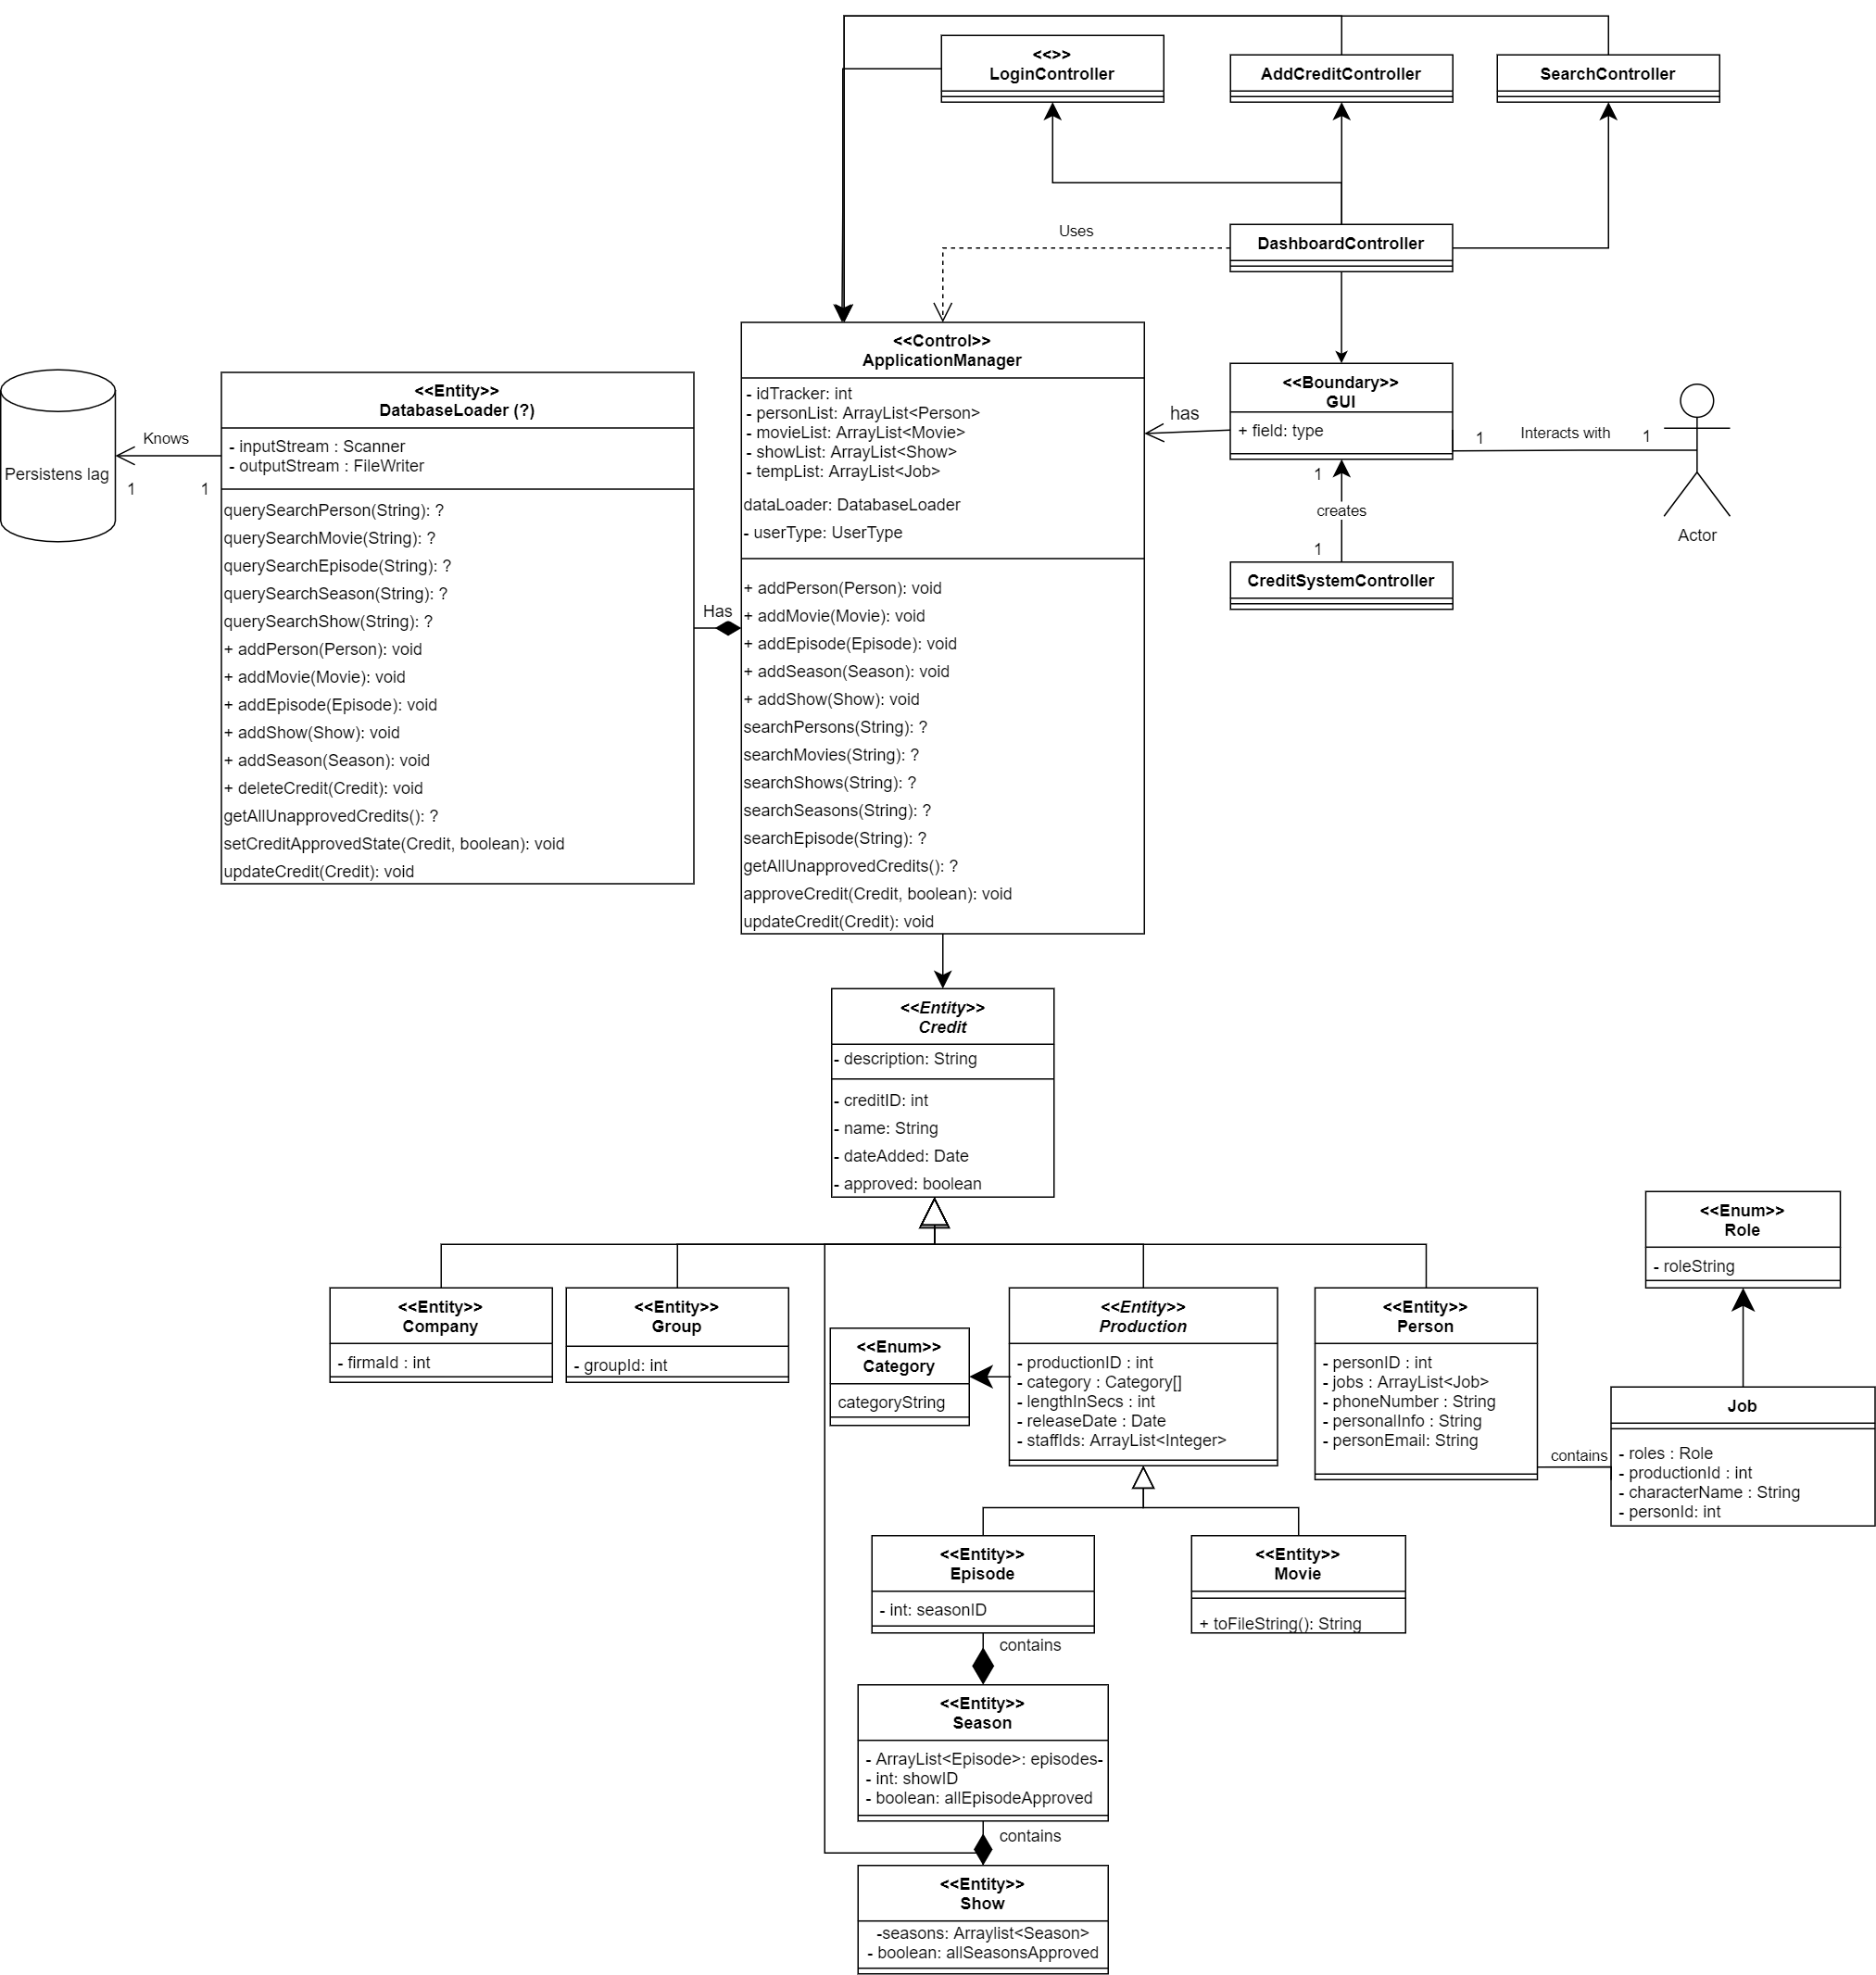
\includegraphics[width=1.2\textwidth]{images/AnalyseKlasseDiagramV3.png}}
    \caption{Endelige analyse klassediagram}
    \label{fig:AnalyseKlasseDiagramV3}
\end{figure}

Klassediagrammet viser at al kommunikation sker gennem ApplicationManager. I første iteration var det nogenlunde denne model der blev fulgt. I overgangen til Iteration 2, gennemgik gruppen dog et større omdesign, for at strukturere programmet for at overholde en bedre softwarestruktur. Bl.a. er ApplicationManager klassen alt for kompleks, og tre-lags-modellen bliver ikke overholdt ordentligt. Denne designprocess gennemgås i designafsnittet herefter. 


% \paragraph{Yderligere brugsmønsterrealisering} De yderligere brugsmønsterrealiseringer er lagt i bilag \textbf{(RET BILAG HER!!!!!!!!!)}


